\documentclass[UTF8,11pt]{ctexart}
% 中文插图 / 表格示例：把 figure.png、figure.jpg 换成自己的图片即可
\usepackage[a4paper,margin=2.2cm]{geometry}
\usepackage{graphicx}
\usepackage{booktabs}   % 三线表
\usepackage{multirow}   % 合并行
\usepackage{tabularx}   % 自动折行的宽表
\usepackage{longtable}  % 跨页长表
\usepackage{subcaption} % 子图
\usepackage{amsmath,amssymb}
\usepackage{float}
\usepackage[hidelinks]{hyperref}

\graphicspath{{./}} % 图片默认目录，也可以写 images/

\title{插图与表格排版示例}
\author{LaTeXStudio}
\date{\today}

\begin{document}
\maketitle

\section{插图}

\subsection{单张图片}

用 \verb|\includegraphics| 插入图片，常用参数有 \verb|width|、\verb|height|、
\verb|scale| 与 \verb|angle|。只给宽度、让高度自适应是最稳妥的做法。

\begin{figure}[H]
  \centering
  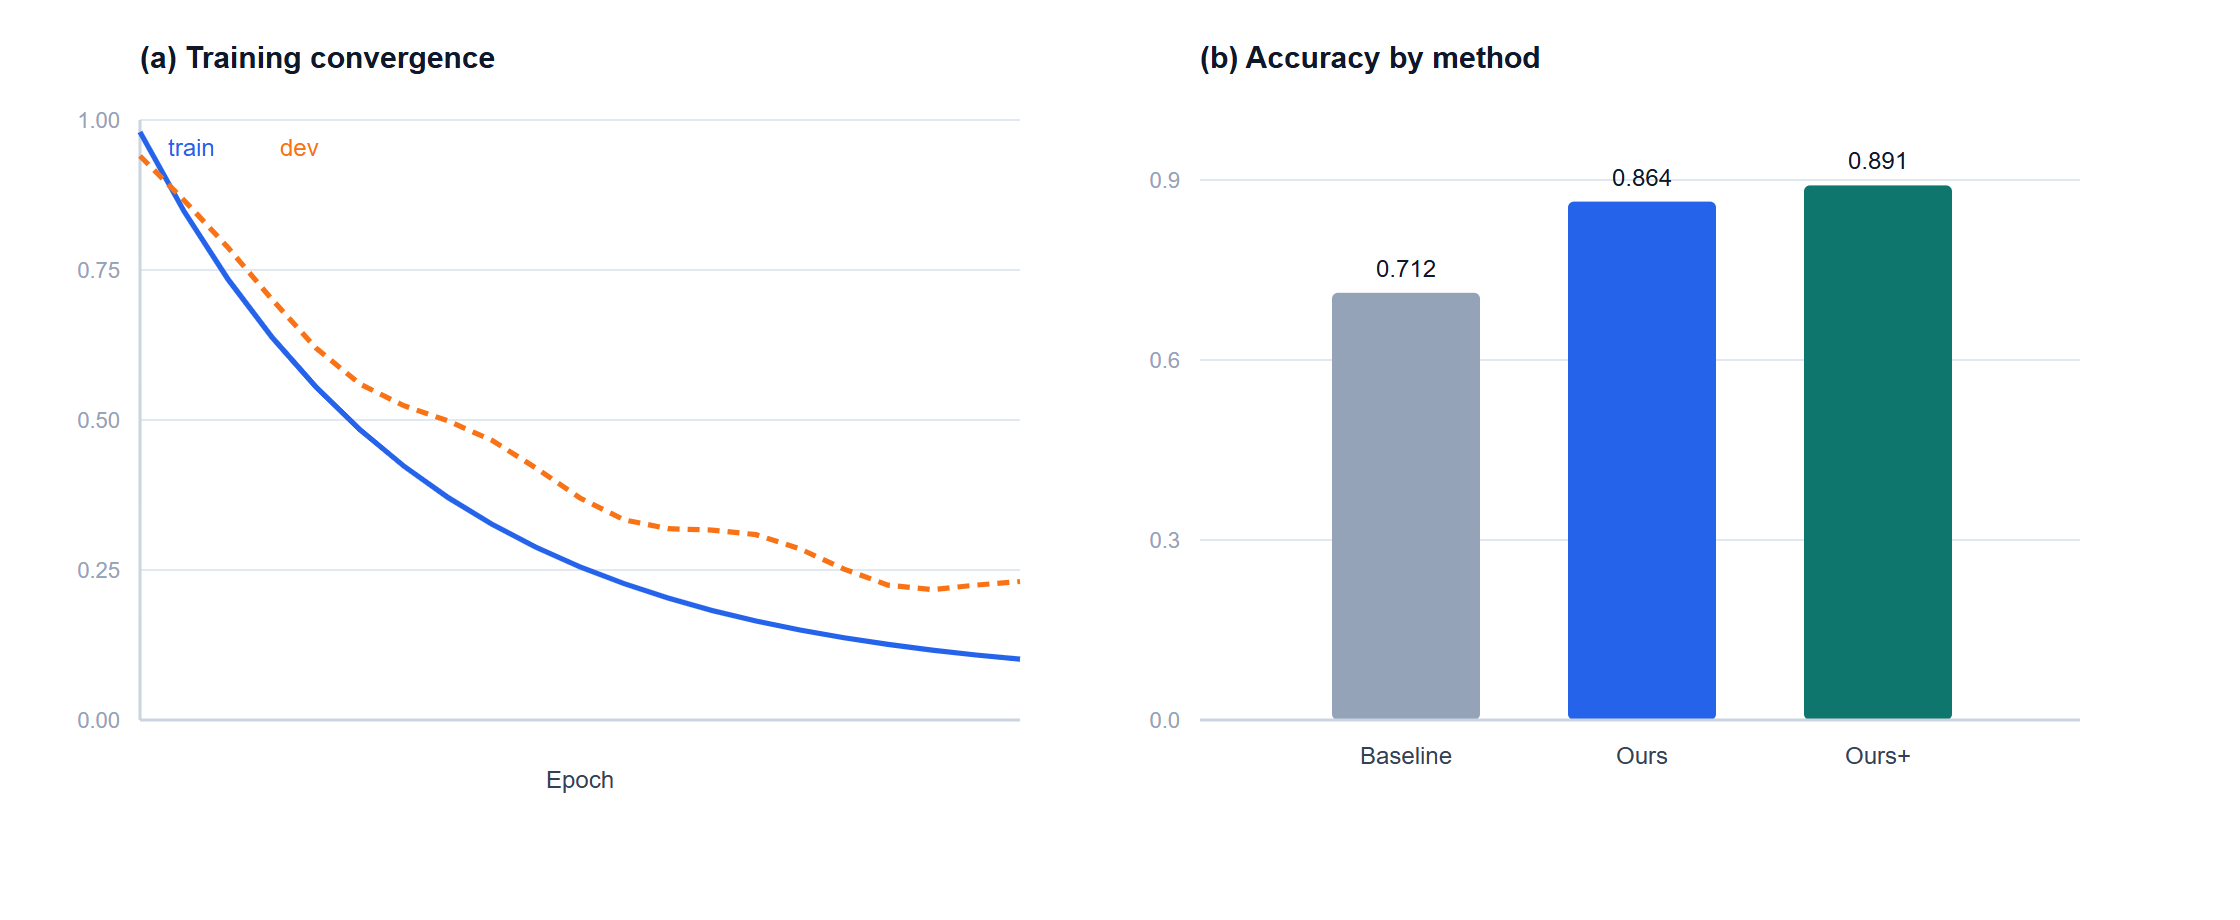
\includegraphics[width=0.8\linewidth]{figure.png}
  \caption{PNG 插图。截图、折线图、柱状图等位图用 PNG；照片用 JPG 体积更小；
    论文里的矢量图更推荐 PDF（\texttt{\textbackslash includegraphics\{fig.pdf\}}）。}
  \label{fig:png}
\end{figure}

\subsection{并排子图}

\begin{figure}[H]
  \centering
  \begin{subfigure}{0.47\linewidth}
    \centering
    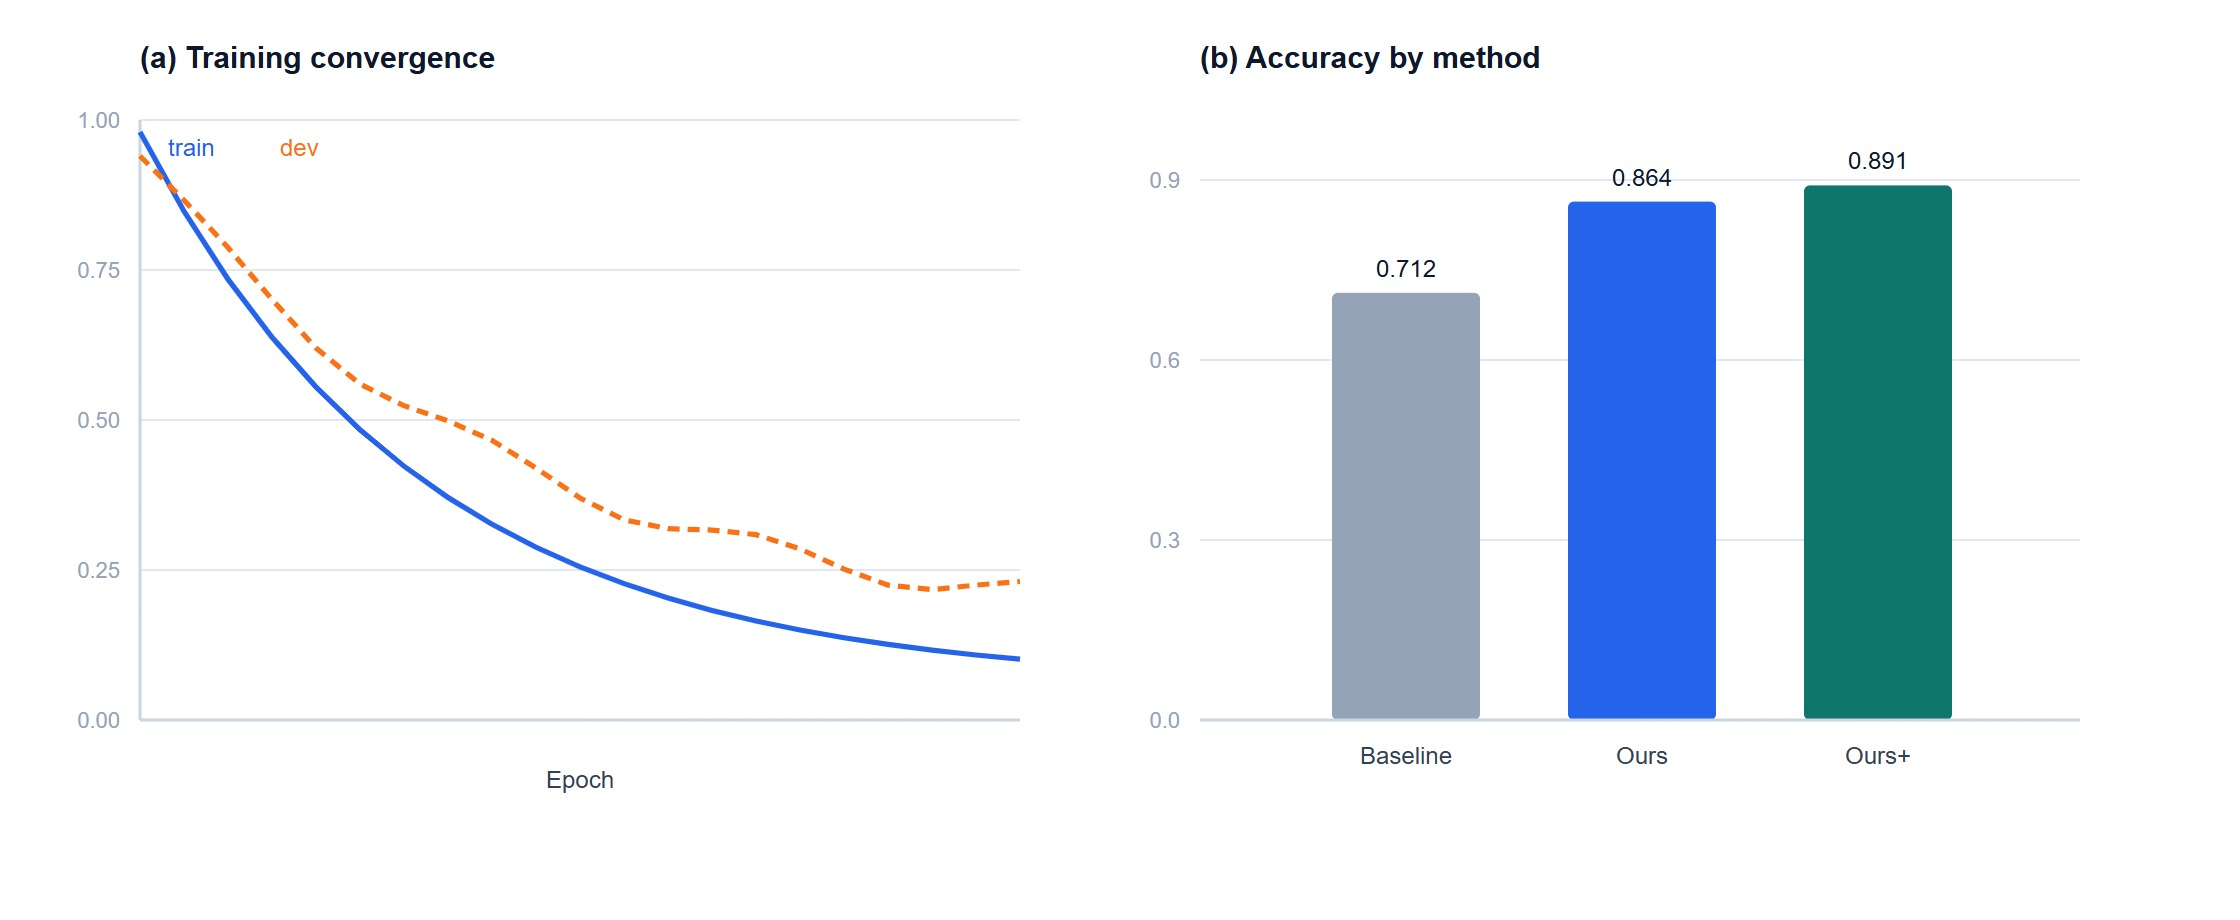
\includegraphics[width=\linewidth]{figure.jpg}
    \caption{JPG 版本}
    \label{fig:sub-a}
  \end{subfigure}\hfill
  \begin{subfigure}{0.47\linewidth}
    \centering
    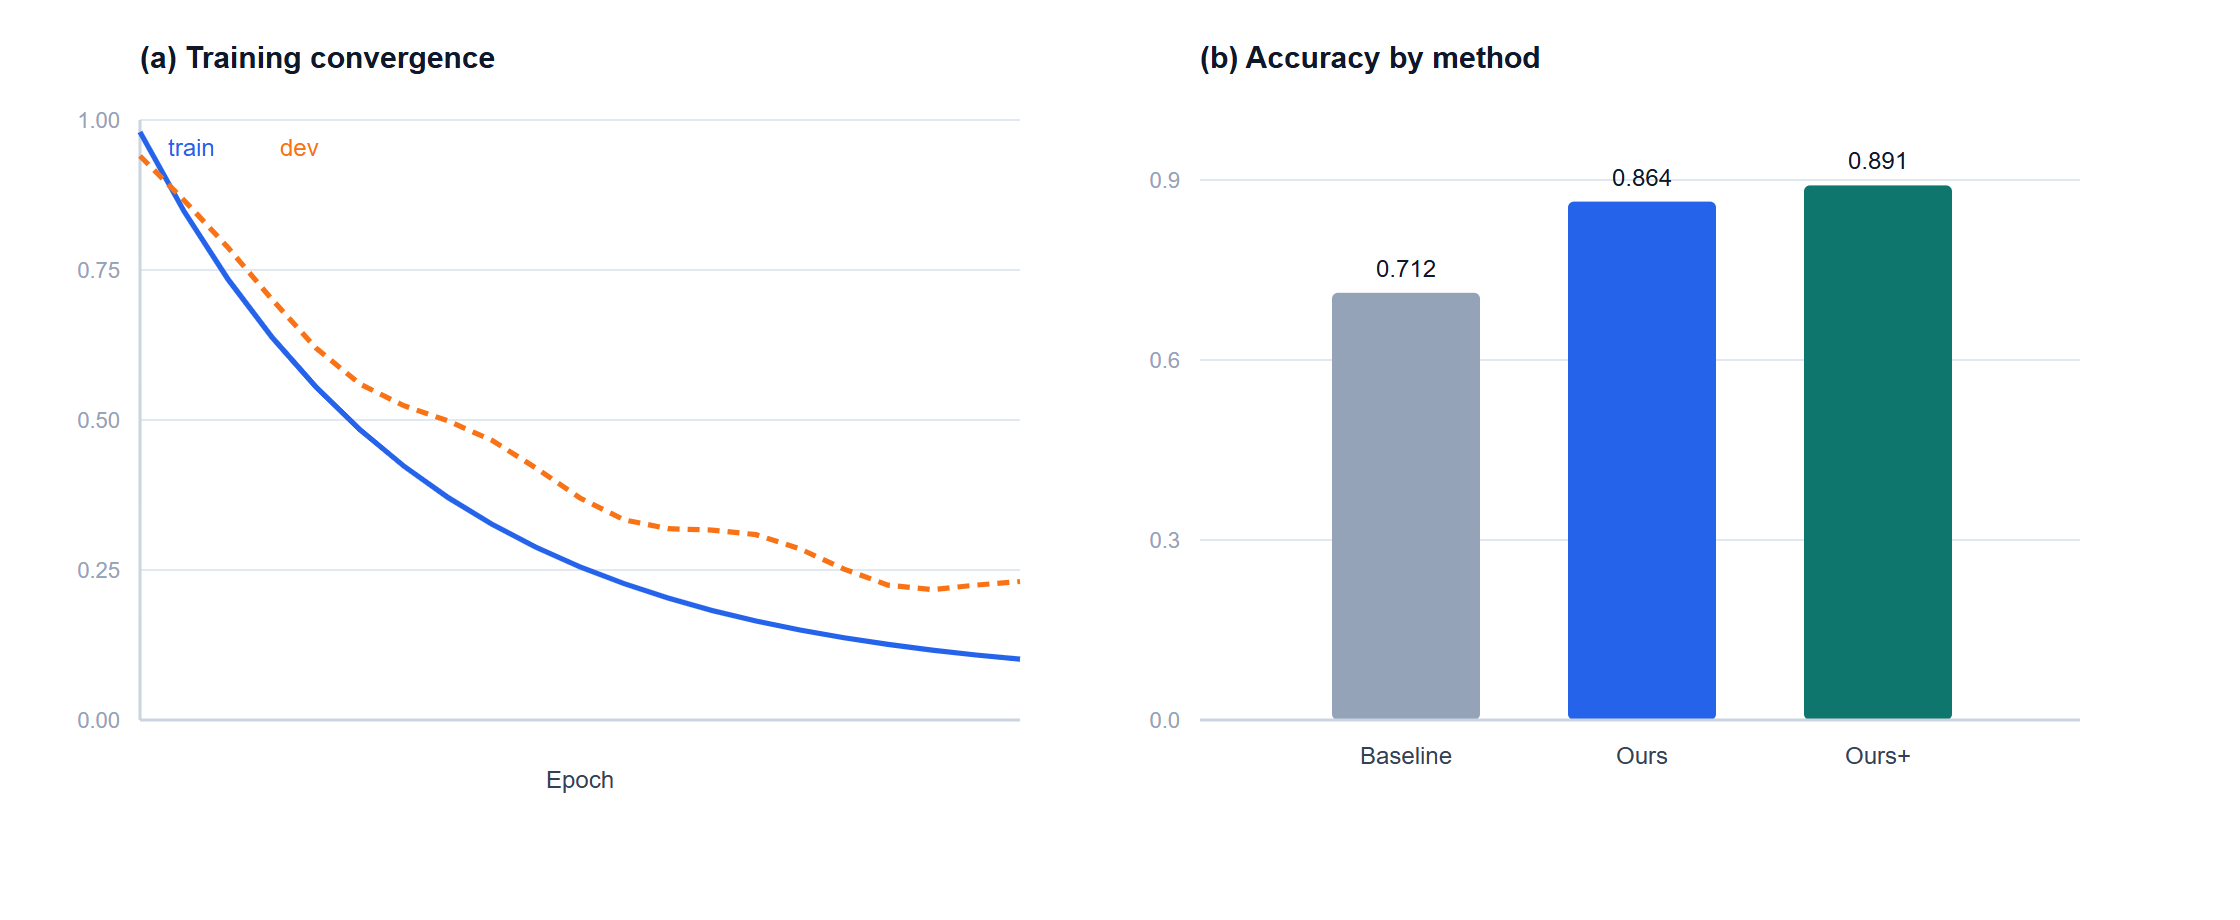
\includegraphics[width=0.72\linewidth]{figure.png}
    \caption{缩小到 72\%}
    \label{fig:sub-b}
  \end{subfigure}
  \caption{子图用 \texttt{subcaption} 宏包，横排时用 \texttt{\textbackslash hfill} 撑开间距。}
  \label{fig:subs}
\end{figure}

\section{表格}

\subsection{三线表}

\begin{table}[H]
  \centering
  \caption{booktabs 三线表（推荐用于正式论文）}
  \label{tab:booktabs}
  \begin{tabular}{lcc}
    \toprule
    方法 & 准确率 & F1 \\
    \midrule
    Baseline & 0.712 & 0.698 \\
    Ours     & 0.864 & 0.851 \\
    Ours+    & \textbf{0.891} & \textbf{0.879} \\
    \bottomrule
  \end{tabular}
\end{table}

\subsection{合并单元格}

\begin{table}[H]
  \centering
  \caption{multirow 纵向合并 + multicolumn 横向合并}
  \label{tab:multirow}
  \begin{tabular}{llcc}
    \toprule
    \multirow{2}{*}{模型} & \multirow{2}{*}{骨干网络} & \multicolumn{2}{c}{准确率} \\
    \cmidrule(lr){3-4}
     & & 验证集 & 测试集 \\
    \midrule
    Ours   & ViT-B & 0.864 & 0.871 \\
    Ours+  & ViT-L & 0.891 & 0.883 \\
    \bottomrule
  \end{tabular}
\end{table}

\subsection{自动折行的宽表}

\begin{table}[H]
  \centering
  \caption{tabularx 让备注列自动换行，宽度撑满版心}
  \label{tab:tabularx}
  \begin{tabularx}{\linewidth}{@{}lXc@{}}
    \toprule
    配置 & 说明 & 耗时 \\
    \midrule
    default & 默认超参数，不做任何数据增强，作为对照基线 & 1.2h \\
    strong  & 打开 RandAugment、MixUp 与标签平滑，训练更久但更稳 & 3.6h \\
    \bottomrule
  \end{tabularx}
\end{table}

\subsection{跨页长表}

\begin{longtable}{@{}cll@{}}
  \caption{长表会自动跨页并重复表头}\label{tab:long}\\
  \toprule
  序号 & 名称 & 备注 \\
  \midrule
  \endfirsthead
  \toprule
  序号 & 名称 & 备注 \\
  \midrule
  \endhead
  \bottomrule
  \endfoot
  1 & alpha & 第一行 \\
  2 & beta  & 第二行 \\
  3 & gamma & 第三行 \\
  4 & delta & 第四行 \\
  5 & eps   & 第五行 \\
\end{longtable}

\section{公式与引用}

行内公式如 $f(x)=\frac{1}{\sqrt{2\pi}\,\sigma}\exp\!\left(-\frac{(x-\mu)^2}{2\sigma^2}\right)$，
编号公式见式~\eqref{eq:loss}，图片引用见图~\ref{fig:subs}，表格引用见表~\ref{tab:booktabs}。

\begin{equation}
  \mathcal{L}(\theta) = -\frac{1}{N}\sum_{i=1}^{N} \log p_\theta(y_i \mid x_i)
  \label{eq:loss}
\end{equation}

\end{document}
